\section{Remote Challenge: 1 vs 1}
\label{sec:OneVsOneChallenge}

\subsection{Idea of the Challenge}
% Patrick
The aim of this challenge is to have a competitive game play given the current situation. 

Two robots play against each other on a full maybe down scaled field. The goal is to shoot balls from the own half into the opponent's half or goal to score points. It is not allowed to leave the own half. Four balls, two on each side, can be shot by the robots.

This challenge focuses on the following aspects:
\begin{itemize}
    \item Remote deployment or fully autonomous setup of NAO software and standardized settings for game play in a remote arena on foreign robots,
    \item Automatic and semi-automatic calibration of NAO (vision, motion, etc.), 
    \item One versus One NAO competition in a ladder KO competition with all teams without much robot interaction. 
\end{itemize}

Requirements to participate in this challenge are, being able to
\begin{itemize}
	\item host an arena, see \ref{sec:c3_BasicRequirementsForArenas}
	\item deploy your robot's software remotely or fully autonomous setup, see \ref{sec:c3_BasicRequirementsForTeams}
\end{itemize}

If teams provide an autonomous setup, all teams can use this to play against this in their own arena. Also teams who cannot host an arena.

\subsection{Prerequisites}
\label{sec:c3_Prerequisites}
% Patrick
For this challenge teams need to fulfil multiple requirements, which are listed below in more detail.

To be able to participate, teams have to deploy their software on the NAO remotely, or you can deliver a fully autonomous \info[]{Is this allowed by SoftBank} setup. There will be several opportunities for the teams to talk, discuss, exchange ideas and code over the next few months until RoboCup. Two options will be properly available: Meetings like RoDEO and a spring RoHOW as well as to discuss on the SPL Discord channel. The second option is a code sharing section like it is available for the V6 support on RC SPL website.

If teams are not able to participate, they (and the other teams as well) can download and deploy the images for fully autonomous setup, calibration and challenge play in the own lab. These games are not part of the ladder system and are outside the competition.

\subsubsection{Basic requirements for teams}
\label{sec:c3_BasicRequirementsForTeams}
\begin{itemize}
    \item A team must be able to deploy their robot software remotely or be able to produce a fully autonomous image for a robot
    \item A team must be able to host an arena. If not, they have to find a substitute team, who takes over their hosting arena responsibilities.
    \item A robot should be able to semi- or fully automatic calibrate itself.
\end{itemize}

\subsubsection{Basic requirements for arenas}
\label{sec:c3_BasicRequirementsForArenas}
Teams have to fulfil the following items to be able to host an arena.

\begin{itemize}
    \item A standard field (see \ref{sec:environment_setup}) that is nearly of the size of an approximately 3/4 field or larger.
	\item Wi-Fi with standard SPL\textunderscore A SSID, standard password (as communicated before the competition via e-mail) and standard IP \texttt{10.0.0.2} address and DHCP turned off
    \item Remote network access via:
    \begin{itemize}
        \item VPN connection,
        \item Mobile connection,
        \item TeamViewer, remote desktop connection or VPN connection from the arena to the remote team
    \end{itemize}
    \item Camera, tablet or laptop for on field online calibration with remote team using Discord
    \item Streaming setup, see~\ref{sec:streaming_setup}
	\item The latest Game Controller running
    \item At least \textbf{two} working NAOs V6 per game
    \item More than \textbf{two} USB Sticks with 16 GB or more memory for flashing and logging 
    \item At least \textbf{four} standard balls
    \item Assistants for remote setup and autonomous setup
    \item Referees (1 Head, 1 Game Controller Operator, $>= 2$ Assistants (Who are also volunteers for the teams in setup phases. They are also in the following game local representative for the teams.))
\end{itemize}

If you cannot fulfil all requirements (equipment or number of people in the field room, etc.) but you would like to host an arena, please contact the TC.

\subsection{Arena and organizational setup}
\label{sec:arean-org-setup}
% Patrick
This challenge relies on a standardized arena setup as well as on exchanging all necessary information. This section provides the description for this.

\subsubsection{Data Exchange}
\label{sec:data_exchange}
Teams exchange data during the days of RoboCup 2021 and before using a Nextcloud drive. An access link and password will be sent to the team leaders and have to be used with care. In the Nextcloud every team has its own folder (team number) which will be used for sharing the following data:

\begin{itemize}
    \item In folder \textbf{field dimensions} each team has to provide a json file (template will be in the root folder of the drive) describing the field dimensions according to the rules (see \ref{sec:field_dim}). The file has to be named \texttt{field\_dimensions.json}. This file has to be uploaded until the \textbf{15th of June 2021}. The file will be used for autonomous setup and game play. To configure the arena the corresponding field dimensions json will be copied on the USB drive after flashing as \texttt{field\_dimensions.json} in the folder configuration. This allows the usage of the same image at different arenas.
    \item  In the folder \textbf{field images} each team has a folder where photos from the arena from different angles and at different day \& night-times with focus on the lighting conditions get uploaded until the 15th of June 2021.
    \item In \textbf{Robot Setup} the arena teams find a binary image for a particular game. Each game has an identifier \textit{Game\_ID} and this identifier has to be used as folder name. The binary image has to be uploaded \textbf{two hours} before the game starts. Next to the image you have to define to configuration folder for the player. The containing files will be copied in the root on the USB drive. The USB drive will be plugged into the robot after flashing. Within this configuration folders you can also place files to configure your image. There is one mandatory file: \texttt{field\_dimensions.json}. This file has to be used by the robot's software.
    \item In \textbf{Arena Access} remote teams find an instruction how to access the arena. Each team must provide team specific credentials and share them with the responsible person in each team until the 1st of June. Every team has to announce a responsible person for credentials and remote setup until the 1st of June. The list of responsible people can be found in the root folder of the Nextcloud drive.
    \item In the root folder you find a \texttt{streaming.md} file where every team has to publish a link that can be used by public to watch the game. It will be used on the SPL website / RoboCup 2021 website as well. Further details for streaming, see~\ref{sec:streaming_setup}.
	\item Logs and images will be uploaded from the hosts into the folder \texttt{Logs/Game\_ID}, where \textit{Game\_ID} is replaced by the game identifier, after the game when bandwidth is available. It is assumed that logs and images are stored on the USB drive attached to the NAO in the folder \texttt{logs}. Other files will be ignored. 

\end{itemize}

\subsubsection{USB Drive}
\label{sec:c3_USB_Drive}
USB drives are used to flash a robot with a binary image or to store data during the game play of the robot.

During the competition a USB drive is used for two purposes:

\paragraph*{Flashing}
A USB Drive is used to flash a robot either with the standard SoftBank image or with a provided one. After flashing, this USB Drive gets replaced by the \textit{storage} USB drive.

\paragraph*{Storage}
After \textit{Flashing} a robot, a robot will be equipped with a storage USB drive with ext3 file system. It will be used for the following purposes:

\begin{itemize}
	\item \textbf{Configuration}: Configuration files, at least \texttt{field\_dimensions.json}, will be copied into the root folder of the USB drive. 
	\item  \textbf{Logging}: If teams want to store log files or images and get them uploaded in the Nextcloud, they can store the files in a \texttt{logs} folder on the USB-Drive. 
\end{itemize}

\subsubsection{Network Setup}
The following section defines network requirements for a local venue that hosts remote games. The network infrastructure should be as transparent as possible for remote participants. It should get as close as possible to an on-site experience. Please also contact your local IT administrators and agree your setup with them.

\paragraph{General}

\begin{itemize}
    \item Participants need easy access to their robots for uploading code and debugging. No ports should be blocked. ICMP must not be blocked. % TODO: Which ports are necessary?
    \item Robots might accumulate a large amount of log files (including images). These logs will be uploaded after games for analysis. Minimum 100Mbit/s (symmetric) is recommended for a venue, favourable 1Gbit/s. Logs can also be uploaded from another network.
    \item To not overwhelm the network, teams should rate limit their network activity (in particular long log downloads and uncompressed video streams from NAOs during debug sessions)
\end{itemize}

\paragraph{SPL Game specific}

\begin{itemize}
    \item Team Messages (SPLStandardMessages) must be receivable for remote participants.
    \item Team Messages must not be forwarded from remote participants to 10.0.0.0/16 (SPL\_A).
    \item GameControllerMessages must be receivable for remote participants.
    \item GameControllerMessages must not be forwarded from remote participants to 10.0.0.0/16 to not allow remote participants to control the game (by accident).
\end{itemize}

\paragraph{Example configuration}

\begin{figure}[ht!]
    \centering
    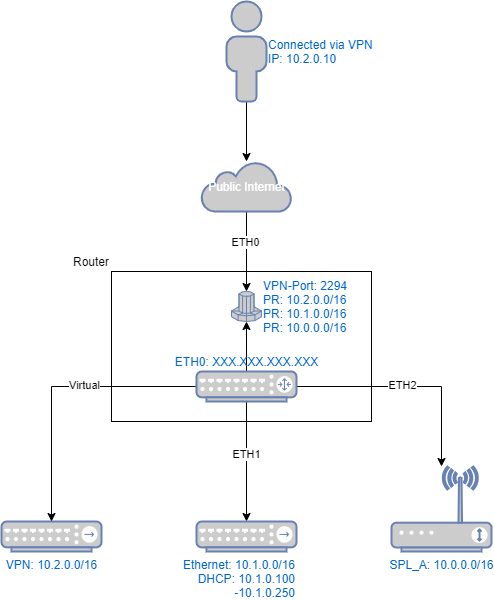
\includegraphics[width=0.5\textwidth]{figs/network.png}
    \caption{Network setup example}
\end{figure}

\begin{itemize}
    \item  The network could be divided for example into three subnets:
    \begin{itemize}
        \item 10.0.0.0/16: The actual SPL\_A wifi network on at least 2.4\,GHz. Each team must use 10.0.TEAM\_NO.2-254 for their robots. GameController will be on 10.0.0.2. DHCP is not active.
        \item 10.1.0.0/16: The ethernet network for robots. Each team must use 10.1.TEAM\_NO.2-254 for their robots. Static addressing is required when robots are assigned to a team. DHCP is active, statically assigning 10.1.0.2-255 to robots that are currently not assigned to any team (pool).
        \item 10.2.0.0/16: The VPN network. Remote participants are assigned to this network and can access the other networks. Team- and GameControllerMessages are forwarded from 10.0.0.0/16 to this subnet. DHCP is active. Broadcasting to other subnets is not possible.
    \end{itemize}
    \item Router (e.g. Ubiquiti EdgeRouter Lite 3-Port Router from Ubiquity \url{https://www.ui.com/edgemax/edgerouter-lite/})
    \begin{itemize}
        \item serves as router for the whole network.
        \item has a globally routable (and accessible) IPv4 address.
        \item hosts an OpenVPN Layer2 VPN Server
        \item opens a network port to allow incoming OpenVPN connections
        \item Every team gets one certificate to authenticate via OpenVPN (multiple connections allowed).
        \item Has broadcast forwarding rules in place to allow VPN users to receive Team-/GC-Messages.
        \item GameController computer is assigned 10.0.0.2/16
        \item \texttt{ETH0} could be connected to your university network and is preferably accessible from the internet on the specific port (please contact your computer centre how to realize such a connection). If this is not possible, please check if you can make this network accessible from remote using a mobile internet connection. Or you provide a PC connected to an island network of this structure were people can access the PC using TeamViewer, remote desktop software, or something similar. 
    \end{itemize}
\end{itemize}

If you have questions or problems to set your local network, please contact the TC via email. There will be also a Discord channel for networking to share configuration files and to solve problems.

\subsection{Remote \& Game Setup}
\label{sec:remote_game_setup}
\subsubsection{Button Interface}
To give volunteers an interface to command autonomous acting robot, the following button interface sequences are defined:
\begin{enumerate}
	\item \texttt{Head button front + Chest button}: Starting the autonomous calibration mode
	\item \texttt{1x Chest button}: Stiff robot
	\item \texttt{All three head buttons}: Unstiff robot
\end{enumerate} 

\subsubsection{Start: 2h before match}

    \begin{enumerate}
        \item Assignment of a volunteer from the host team for each remote team. Create own Discord-channel for communication during the whole setup and game phase.
		\item For each team one randomly selected functional robot is assigned from the pool
        \item Connect robot to LAN and power line
        \item Each robot gets flashed 
        \begin{itemize}
            \item with the standard SoftBank binary image.
            \item with the image provided by the respective team.
		\end{itemize}
		\item Each robot gets equipped with a USB drive according to \ref{sec:c3_USB_Drive} and started.
        \item Teams can set their robot up remotely, if necessary. To reduce the amount of data transferred to set the robot up, teams should reduce this as much as they can and use images.
        \item The IP address given by the DHCP Server has to be communicated from the local host to the remote team using Discord.
        \item Dress robots with jerseys.
    \end{enumerate}

\subsubsection{Calibration / Testing: 1 hour before match}
    \begin{enumerate}
        \item 20 minutes to calibrate the robot supported by one volunteer.
        \item Autonomous setup is conducted in the following way: The volunteer place the robot on the normal initial position at the field side. Then the front head button plus the chest button gets pressed to initialize auto calibration mode~(see~\ref{sec:robot_states}). The robot than can move over the whole field to calibrate itself. The robot has 5 minutes to calibrate. At the end of the calibration period, the robot may sit down and get unstiffed. Otherwise the robot will be unstiffed by the volunteer by pressing all head buttons simultaneously~(see~\ref{sec:robot_states}). 

        \item  Check Wi-Fi and game controller connection
    \end{enumerate}

\subsubsection{Game Setup}

	\begin{enumerate}
		\item Robots are in the game controller
		\item Robots sit on field on the game controller's side on their halves on the height of the penalty spot facing the field. With one button press on the chest button the robot has to get up stiffed in the upright position and is waiting for the ready signal from the game controller.
		\item The game will be started using the game controller as \textit{Play-off game} and the robot moves to its starting position.
		\item In \texttt{Set} the balls will be placed and the game will be started using a whistle.
		\item In the second half the robots switch their sides.
		\item Referees apply rules in the direction to prevent hardware damages, because there is no SoftBank Robotics support.
		\item When robots receive the finish message they have to sit down and will be brought to the chargers and plugged into network.
	\end{enumerate}
	
\subsubsection{After Game}
	
	\begin{enumerate}
		\item After, robots received the finish signal of the second half they sit down.
		\item Robots have time to do all post-processing, storing the logs and shutting down.
		\item If robots are not switched off after 5 minutes they will be switched off manually.
		\item The data from the USB drive will be stored on another device and as soon as possible uploaded in the Nextcloud.
		\item Teams are not allowed to download their logs directly.
		\item Robots will be returned to pool for the next game.
	\end{enumerate}


\subsection{Rules}
%Arne
A brief summary of the rule changes will be given here:

\subparagraph{Competition Execution:}
\begin{itemize}
	\item The competition consists of three parts, the first half, a half-time break, and the second half. Each half is 5 minutes counted from the initial kick-off. (\cf Section~\ref{sec:game_struct})
	
	\item Only hardware changes are allowed! In particular, it is permitted to change batteries, fix mechanical problems, reboot the robots. Since the teams are not on site, the assistant referees take over these tasks as if they were a member of the corresponding team. (\cf Section~\ref{sec:game_struct} and Section~\ref{sec:request_for_pickup})
	
	\item Each team has one NAO V6 and by default the two robots are wearing ``home'' and ``away'' jerseys with the number 2 on it (\cf Section~\ref{sec:field_players})
	
	\item The players can be positioned anywhere within their own half, but no player is allowed to touch or exceed the centre / halfway line. (\cf Section~\ref{sec:kick-off} and Section~\ref{sec:leaving_field})
	
	\item There is no manual placement of any robot.(\cf Section~\ref{sec:kick-off})
	
	\item The two balls, for each side, are placed onto the corners of the goal box - goal free kick positions - (\cf Section~\ref{sec:kick_in})
	
	\item If a ball goes over a sideline then the assistant referee will replace the ball back on the point of that sideline where it went out. If the ball goes over an end-line then the assistant referee will replace the ball onto the corner of the goal box. (\cf Section~\ref{sec:kick_in})
	
	\item This competition is executed with a GameController and the use of the button interface as a replacement for any GameController commands is not allowed! (\cf Section~\ref{sec:robot_states})
	
	\item If a player (from both sides) scores a valid goal the ball gets replaced by the referees to one of the starting points, on the other half. The ball is placed farthest away from the player in this half and can then directly be played again. (\cf Section~\ref{sec:goal})
	
	\item After the game is in the state playing, the game state remains in it regardless of shot goals or scored points! Exception are the application of the Global Game Stuck rule and a referee timeout. (\cf Section~\ref{sec:game_stuck:global})
	
	\item A Global Game Stuck is applied if, among other things, no ball was played from one half to the other for more than 1 minute. (\cf Section~\ref{sec:game_stuck:global})
		
	\item Alleine auf dem Feld	
		
	\item Fields that are at least 3/4 of the original size can also be used for this competition. However, field sizes smaller than the original should be reported by email to the TC by June 1, 2021. (\cf Section~\ref{sec:field_dim})
\end{itemize}

\subparagraph{Referees:}
\begin{itemize}
	\item All referees are allowed to \textbf{prevent robots from crashing} to the ground by catching them beforehand and then laying them down gently! (\cf Section~\ref{sec:judgment}) 
	
	\item The head referee decides whether a robot excessively damages itself and should remove it from the field via ``Request for Pick-up''. (\cf Section~\ref{sec:damage_robot})
	
	\item A robot which is unable to autonomously stand up within 20 seconds after a fall and be \textbf{at least 10 seconds upright} will be penalized as fallen robot. (\cf Section~\ref{sec:fallenrobots})
	
	\item Since teams are playing with robots from other teams, there is a \textbf{maximum of 3 hardware related penalties}:
		\begin{itemize}
			\item \textbf{fallen robot} or \textbf{inactive robot}, \cf Section~\ref{sec:fallenrobots}
			\item \textbf{request for pick-up} in the Playing or Ready state - either by the team or by the head referee, \cf Section~\ref{sec:request_for_pickup} and Section~\ref{sec:damage_robot}
		\end{itemize}
		After that this robot is excluded for the rest of the competition!
	
	\item If it comes to an excluding of a robot, the head referee, in consultation with the two team leaders, must decide whether the hardware errors that occurred were exclusively self-inflicted due to faulty code or whether it was a general hardware problem with the robot.
	
	\item Depending on this decision:
	\begin{itemize}
		\item In case of self-inflicted hardware problems will the game continue without this robot till the end of the regular time or till the remaining robot scores more points or has more point scored as the excluded robot. 
		\item For general hardware-related errors of the robot, it will be replaced by another robot and the game will be restarted as soon as possible which depends on how much time this team needs to flash, setup and recalibrate the robot. This must not take longer than the official time for a remote setup (\cf Section~\ref{sec:remote_game_setup})!
	\end{itemize}
	\item A robot exchange can take place at most once per team, in this case this competition would be restarted 2 times! (\cf Section~\ref{sec:forbidden_act})
\end{itemize}

A detailed description of the rules can be found here: Section~\ref{sec:Common_rules}

\subsection{Scoring}
% Arne
\label{sec:scoring}

For this challenge points can be scored by:
\begin{itemize}
	\item Shooting the ball in the opponents half (1 Point)
	\begin{itemize}
		\item The ball has to stop inside the field (\cf Section~\ref{sec:inside_outside})!
	\end{itemize} 
	\item Shooting a goal (1 Point)
	\begin{itemize}
		\item Afterwards the team which scored the goal gets this ball back (\cf Section~\ref{sec:goal})
	\end{itemize}
\end{itemize}

If the defending/other robot touches the ball when it was kicked over the centre line and before it comes to a full stop then \textbf{NO} points are rewarded! This allows the defending team to intercept balls which are shoot into their half of the field.

The head referee has to call:
\begin{itemize}
	\item ``Point for \textless colour\textgreater'' for each scored point.
	\item ``Goal for \textless colour\textgreater'' for each scored goal.
\end{itemize}
and then the points will be counted by the operator of the GameController.
%TODO: either by writing it down or by using a modified GameController

For teams playing with an \textbf{autonomous player} (\cf Section~\ref{sec:c3_Prerequisites}) a multiplication factor of \textbf{1.5} is given. This factor is used at the end of the game and the scored points, for this team, are multiplied by it to calculate the final points (\cf Section~\ref{sec:rankings}). 
%\emph{Note that the resulting points should be rounded to the nearest integer.}

\subsection{Challenge execution}
% Arne
The 1vs1 Challenge is played as a knock-out competition, as the points scored between individual games are not directly comparable. 

The clock stops during stoppages of play (such as ready and set state after global game stuck)!

\subsubsection{Competition System}
It is planned to divide the participating teams into three groups, so that there are 8 teams in each group. Within each group, a ladder system will be used where only the winner of the game will advance. 

In the end there will be 3 winners from each group, who will determine their final placing in matches each against each other. If there is a draw between the three final teams, the points scored in the final matches will be used to determine a winner.

The teams are randomly assigned to the groups and no subdivision into challenger shield or champions cup teams is considered.
To allow all teams to play at least 3 times, the losers of a match will play in additional ladders.

The exact determination of the multiple knock-out rounds/ladders can only be done when the number of participating teams is known and will therefore be announced shortly before the RoboCup. Also the different time zones have to be taken into account and therefore there should only be two games per day per arena.
    
\subsubsection{Winner and Rankings}
\label{sec:rankings}

The team which scored more points than the other, after the expiration of the regular playing time and by applying the multiplication factor, is the winner of the match. If the two teams scored the same number of points, the game will be a draw. In case of a draw the game duration gets extended by one minute. After each extension the (multiplied) score is evaluated again. At max 5 extensions à 1 minute are allowed. \\
If the game is still tied after overtime, a coin is tossed to determine a winner!    
